%%%%%%%%%%%%%%%%%%%%%%%%%%%%%%%%%%%%%%%%%
% University Assignment Title Page 
% LaTeX Template
% Version 1.0 (27/12/12)
%
% This template has been downloaded from:
% http://www.LaTeXTemplates.com
%
% Original author:
% WikiBooks (http://en.wikibooks.org/wiki/LaTeX/Title_Creation)
%
% License:
% CC BY-NC-SA 3.0 (http://creativecommons.org/licenses/by-nc-sa/3.0/)
% 
% Instructions for using this template:
% This title page is capable of being compiled as is. This is not useful for 
% including it in another document. To do this, you have two options: 
%
% 1) Copy/paste everything between \begin{document} and \end{document} 
% starting at \begin{titlepage} and paste this into another LaTeX file where you 
% want your title page.
% OR
% 2) Remove everything outside the \begin{titlepage} and \end{titlepage} and 
% move this file to the same directory as the LaTeX file you wish to add it to. 
% Then add \documentclass[12pt]{article}
\usepackage[english]{babel}
\usepackage{amsmath}
\usepackage{graphicx}
\usepackage{textcomp}
\usepackage{parskip}
\usepackage[colorinlistoftodos]{todonotes}
\usepackage{csquotes}
\usepackage{float}
\usepackage[backend=biber,style=ieee]{biblatex}
\addbibresource{bibliography.bib}

\begin{document}

\begin{titlepage}

\newcommand{\HRule}{\rule{\linewidth}{0.5mm}}
\center 

\textsc{\LARGE Iowa State University }\\[1.5cm] 
\textsc{\Large Center for Statistics and Applications in Forensic
Evidence
}\\[0.5cm] 

\HRule \\[0.4cm]
{ \huge \bfseries Shoe Print Data Collection: Additional Methods }\\[0.4cm] 
\HRule \\[1.5cm]



\begin{center}
\centering
 
\includegraphics[scale=.4]{csafe-logo}\\[1cm]
\end{center}







\end{titlepage}

\section{Introduction}

 When developing the methodology for the longitudinal shoe study conducted by the Center for Statistics and Applications in Forensic Evidence (CSAFE), collection procedures were designed to obtain the most ideal shoe-sole impression possible. While these images will be useful to the researcher and practitioner communities, they do not provide realistic examples of prints that would be collected from a crime scene/suspected crime scene. For this reason, CSAFE researchers have compiled this manual which contains procedures for further data collection and offers new, or edited, procedures that better represent the practices of current forensic examiners and crime scene teams. If at any time there is a question on any of these procedures, please make a note using a post-it note and e-mail the principal investigator, the project manager, the faculty in charge of the study, or the author of the specific procedure. 

\end{document} to your LaTeX file where you want your
% title page.
%
%%%%%%%%%%%%%%%%%%%%%%%%%%%%%%%%%%%%%%%%%
%\title{Title page with logo}
%----------------------------------------------------------------------------------------
%	PACKAGES AND OTHER DOCUMENT CONFIGURATIONS
%----------------------------------------------------------------------------------------

\documentclass[12pt]{article}
\usepackage[english]{babel}
\usepackage[utf8x]{inputenc}
\usepackage{amsmath}
\usepackage{graphicx}
\usepackage[colorinlistoftodos]{todonotes}

\begin{document}

\begin{titlepage}

\newcommand{\HRule}{\rule{\linewidth}{0.5mm}} % Defines a new command for the horizontal lines, change thickness here

\center % Center everything on the page
 
%----------------------------------------------------------------------------------------
%	HEADING SECTIONS
%----------------------------------------------------------------------------------------

\textsc{\LARGE Iowa State University}\\[1.5cm] % Iowa State University 
\textsc{\Large CSAFE}\\[0.5cm] % CSAFE
\textsc{\large Center for Statistics and Applications in Forensic Evidence }\\[0.5cm] % Center for Statistics and Applications in Forensic Evidence 

%----------------------------------------------------------------------------------------
%	2D Shoe Scanner Procedure
%----------------------------------------------------------------------------------------

\HRule \\[0.4cm]
{ \huge \bfseries Mat Scanner Procedure  }\\[0.4cm] % Title of your document
\HRule \\[1.5cm]
 
%----------------------------------------------------------------------------------------
%	AUTHOR SECTION
%----------------------------------------------------------------------------------------

\begin{minipage}{0.4\textwidth}
\begin{flushleft} \large
\emph{Author:}\\
James \textsc{E. Kruse} % James E. Kruse
\end{flushleft}
\end{minipage}
~
\begin{minipage}{0.4\textwidth}
\begin{flushright} \large
\emph{Supervisor:} \\
Dr. Guillermo \textsc{Basulto-Elias} % Supervisor's Name
\end{flushright}
\end{minipage}\\[2cm]

% If you don't want a supervisor, uncomment the two lines below and remove the section above
%\Large \emph{Author:}\\
%John \textsc{Smith}\\[3cm] % Your name
%----------------------------------------------------------------------------------------
%	LOGO SECTION
%----------------------------------------------------------------------------------------

\includegraphics[scale=.5]{Logo}\\[1cm]


\begin{center}
\begin{tabular}{ c   |   c } 
\end{tabular}
\end{center}


%----------------------------------------------------------------------------------------
%	DATE SECTION
%----------------------------------------------------------------------------------------

{\large \today}\\[2cm] % Date, change the \today to a set date if you want to be precise

%----------------------------------------------------------------------------------------

\vfill % Fill the rest of the page with whitespace

\end{titlepage}




\section{Introduction}

The following is the recommended procedure for taking scans using the HR Mat Scanner (Figure 1) from Tekscan.Please note, at no time should the scanner be bent or stored on its side. The mat must remain flat, on a hard surface at all times. 

\begin{figure}[!htp]
\centering
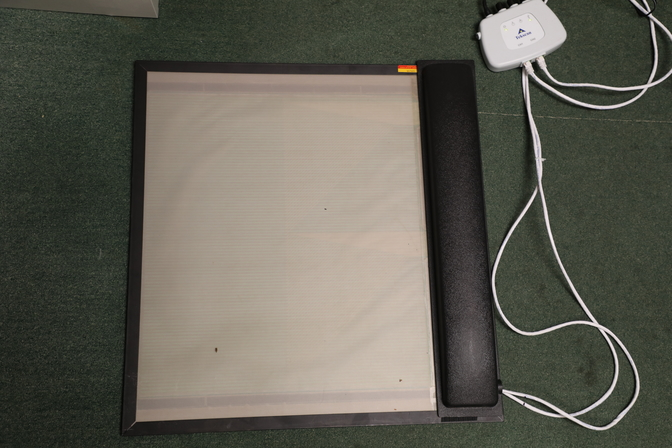
\includegraphics[scale=0.35]{Mat}
\caption{Tekscan Mat Scanner}
\label{Image 1}
\end{figure}

NOTE: You do not need to worry about a still image. Just follow this procedure and the image will generate from the video.

\subsection{Procedure}

1.	Place the scanner on the ground away from anything that could fall on it. There should be sufficient room both in front and in back of it for a participant to walk up and away. Follow the written instructions in the manual for exact set up procedures. Many of the pieces are quite sensitive. 

Note: If software needs to be installed, please call IT. 



2.  Using masking tape, create a path for the participants to walk on. The path is labeled in that whatever foot you want scanned, step on the boxes labeled for that side (ie. you want to scan the right foot, step on the boxes labeled "right").   
 
3. Select the "FootMat Research 7.10" icon on the desktop of the lab computer. A gray selection box will appear (Figure 2). Select the participant "Subject Subject" and click "open patient" for details/previous videos. Due to the files later being saved to the computer and labeled with the participants ID number, the same "patient" will be used for each participant.

\begin{figure}[!htp]
\centering
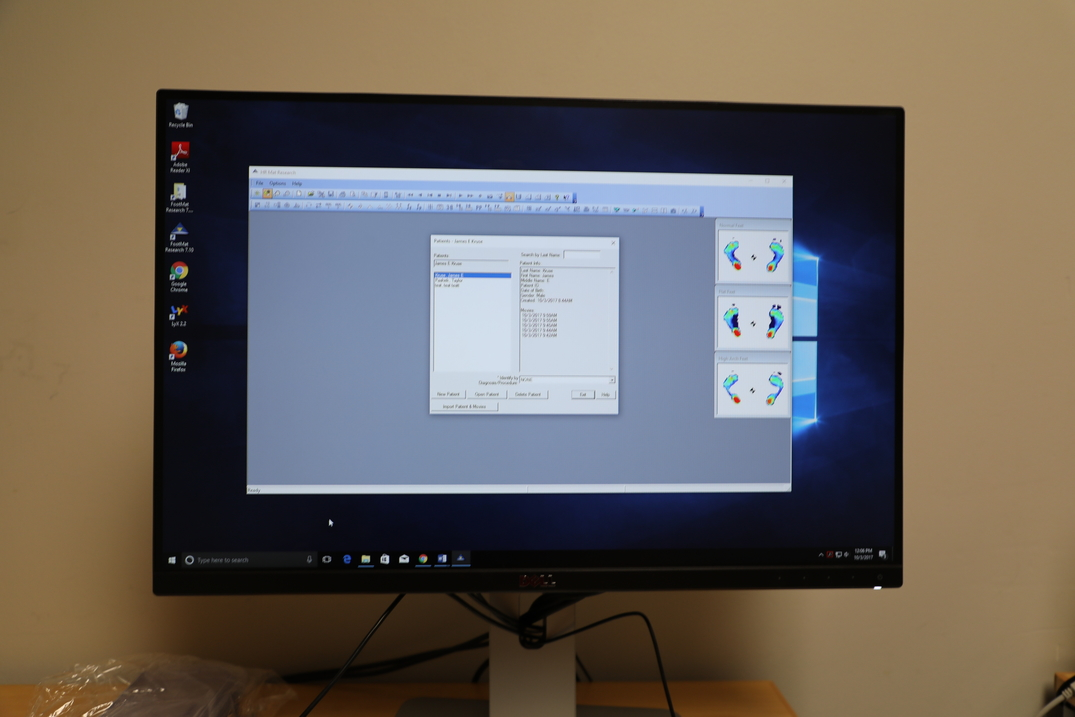
\includegraphics[scale=0.25]{Mat_Screen_1}
\caption{Opening screen on the computer desktop}
\label{Image 2}
\end{figure}

4. Have the participant put on a pair of the disposable socks before they step onto the mat scanner. This will eliminate the variation between people's socks and keep them from stepping barefoot onto the scanner. 

5. When the technition is ready, (Figure 3) make sure that the participant is standing at the beginning of the pre-set path. The order of scans will start with right bare foot and then proceed in the same order that is given on the key (see front cover). Press the red record button on the second tool bar. Have the participant step onto the scanner. They should step on (Figure 4) as if taking a normal step and then step back off (Figure 5) making sure to get only the designated foot on the scanner. 

\begin{figure}[!htp]
\centering
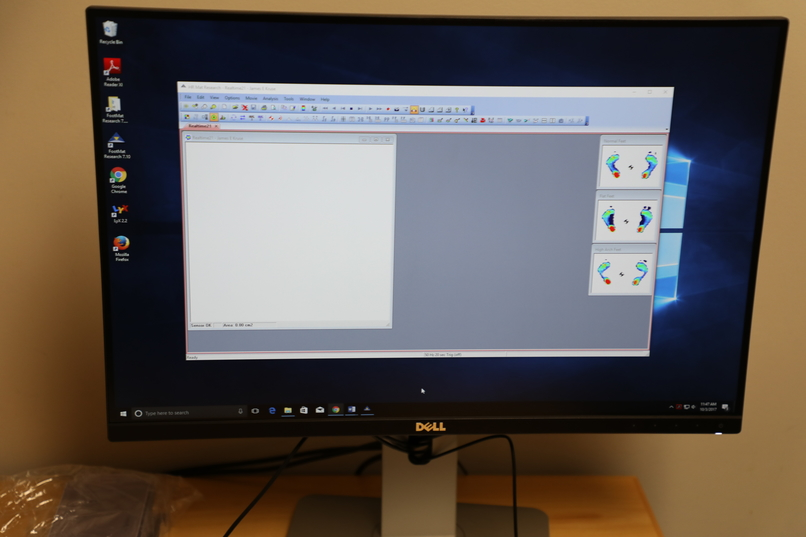
\includegraphics[scale=0.32]{Mat_Clear}
\caption{Clear screen on the computer desktop}
\label{Image 3}
\end{figure} 

\newpage

\begin{figure}[!htp]
\centering
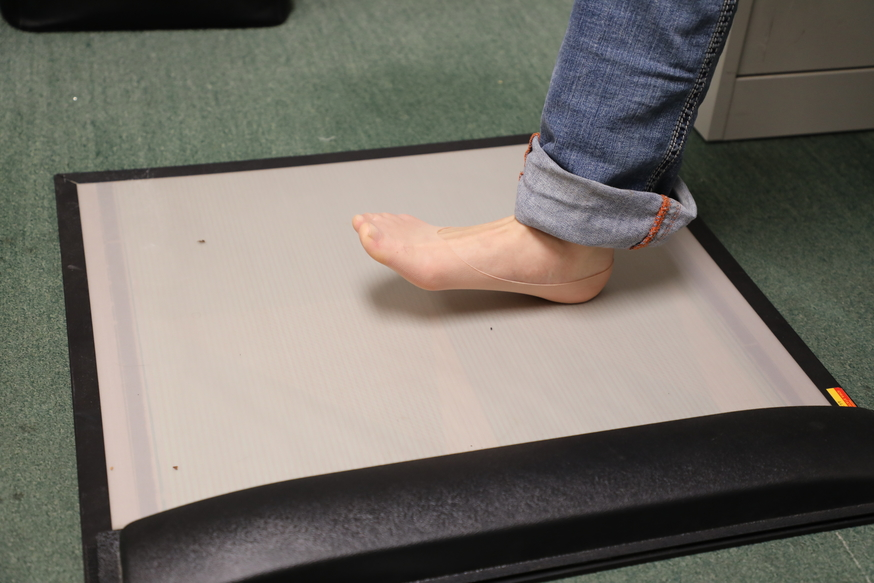
\includegraphics[scale=0.28]{Mat_Step_1}
\caption{Participant stepping onto the Mat Scanner}
\label{Image 4}
\end{figure}


\begin{figure}[!htp]
\centering
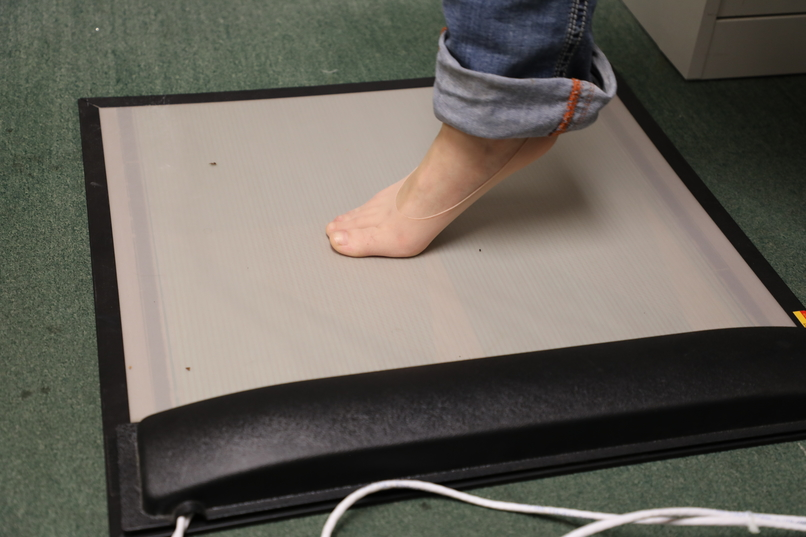
\includegraphics[scale=0.3]{Mat_Step_2}
\caption{Participant stepping off of the Mat Scanner}
\label{Image 5}
\end{figure}

\newpage

Note: If you wish to have a larger window for the participant to step onto the scanner, select options on the first tool bar. Then select 3-Box Analysis.  Please see Figures 6-8 for examples of a barefoot scan and a shoe scan. 

\begin{figure}[!htp]
\centering
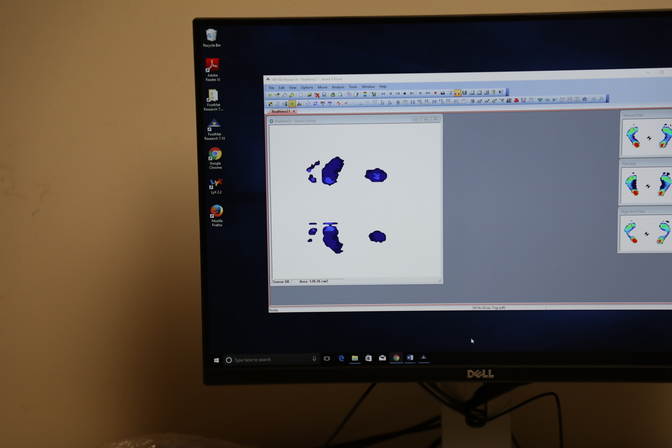
\includegraphics[scale=0.4]{Mat_Scan}
\caption{partial scan}
\label{Image 6}
\end{figure}

\begin{figure}[!htp]
\centering
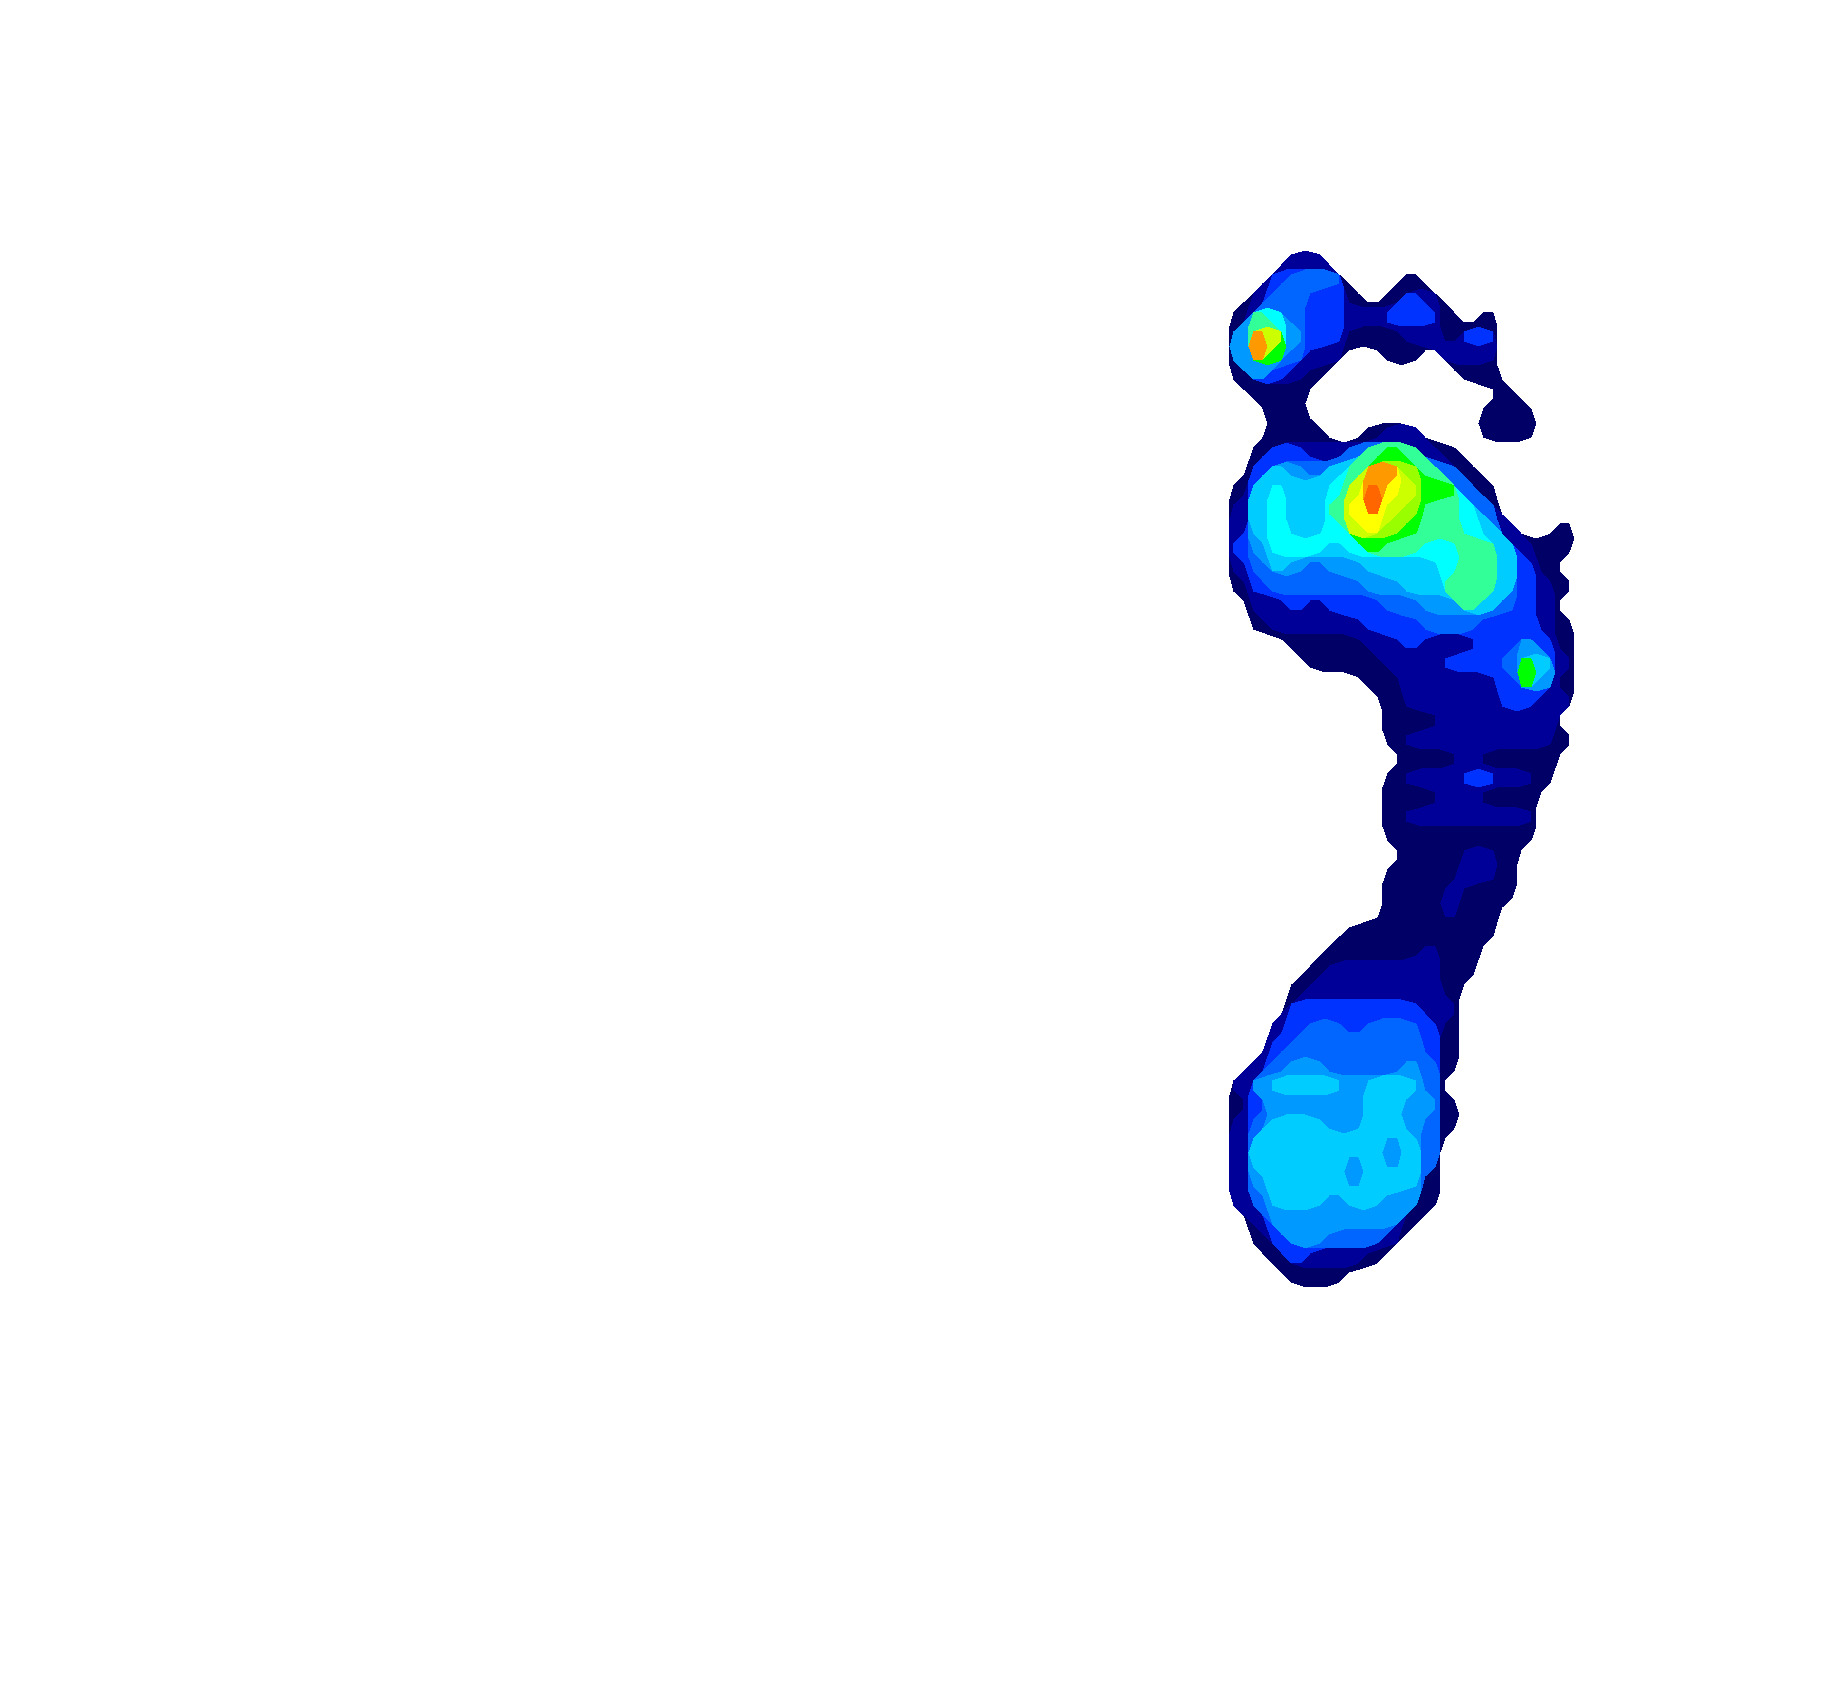
\includegraphics[scale=0.15]{Mat_Foot}
\caption{Participant stepping off of the Mat Scanner}
\label{Image 7}
\end{figure}

\begin{figure}[!htp]
\centering
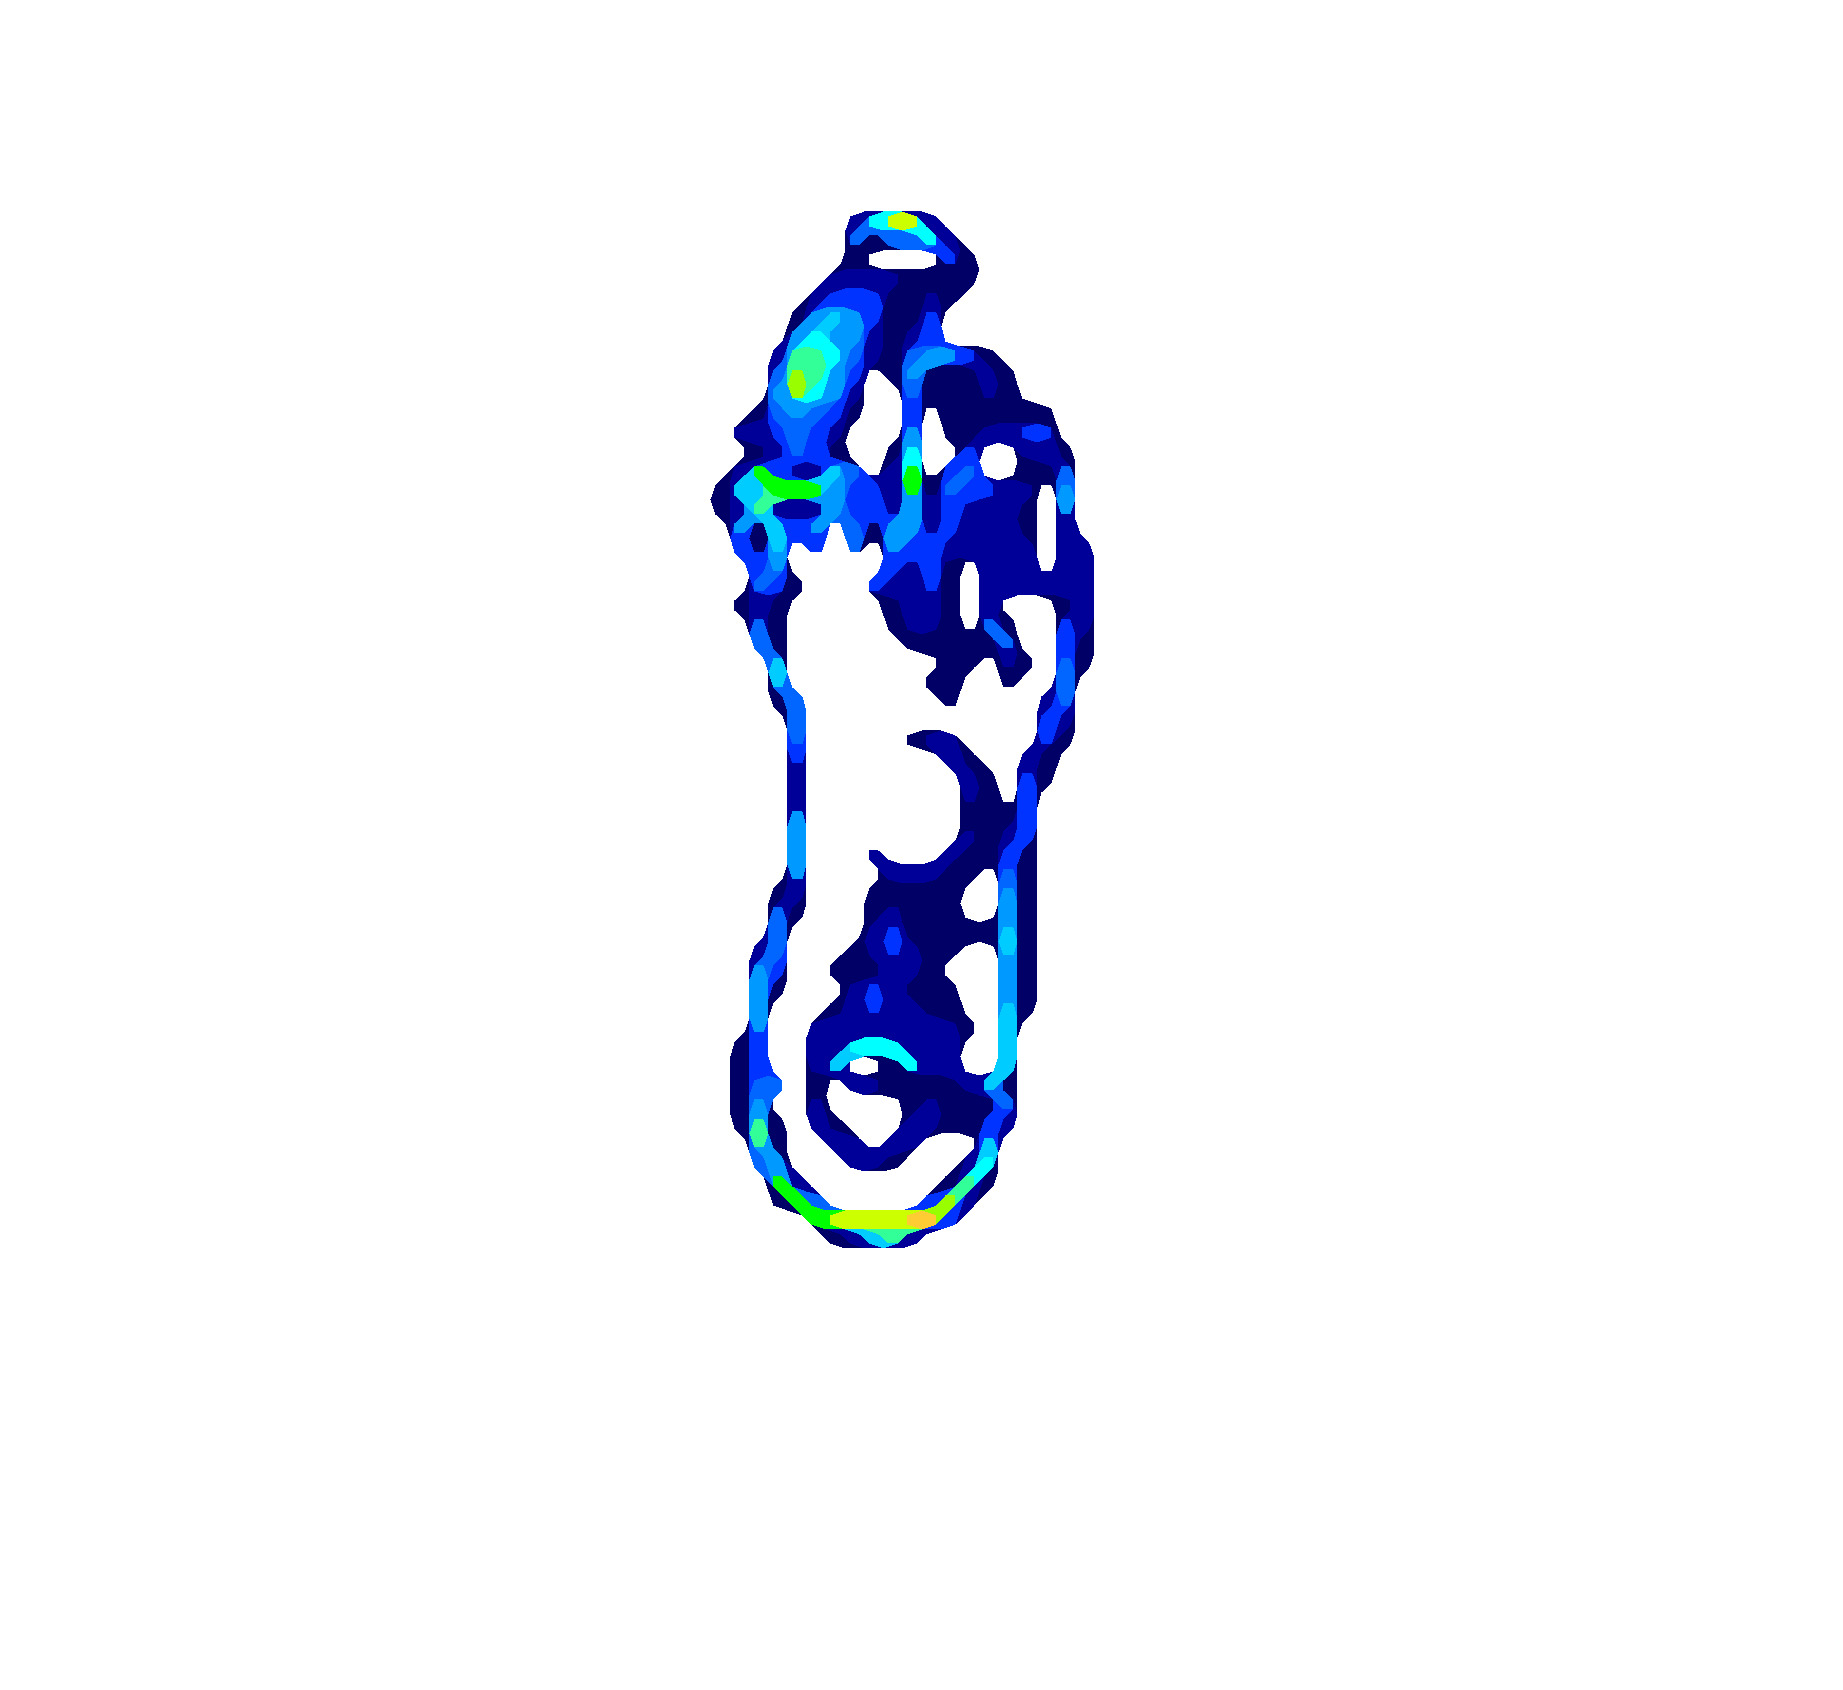
\includegraphics[scale=0.15]{Mat_shoe}
\caption{Participant stepping off of the Mat Scanner}
\label{Image 8}
\end{figure}

\newpage

6. At this time, the tech will save the recording to be analyzed at a later time. To do this, you will go file "save movie as" and name the file according to the Shoe Image Filename Generator. Image 5 will be used for each of the individual repetitions. The should be saved under the (:Z) Drive on the laptop computer. In the (:Z) Drive there will be a folder named: Cohort "Number" Initial Matscan. Within that folder there is a sub folder titled Movie Recordings and that is the save location.  

7. The process will then be repeated for each repetition for the participant barefoot and with shoes. 


NOTE: ALWAYS DOUBLE CHECK THE NAMING KEY ON THE BACK OF THE MANUAL COVER!!!


\subsection{Saving the desired files from the previously recorded movie:}

1. Open the HR MAt Research Program. Go to file "open movie" and select the desired file to be manipulated. select NO when prompted to do so. 

***generate name***

2. First you need to save the file as an an AVI (50 frames a second). When prompted, select "full frames uncompressed". Browse and find the file location. Name the file according to the Shoe Image Filename Generator. Image 1 will be used for each of the individual repetitions. The should be saved under the (:Z) Drive on the laptop computer. In the (:Z) Drive there will be a folder named: Cohort "Number" Initial Matscan. Within that folder there is a sub folder titled Required Files and that is the save location.  Select "OK". 

2.Then you will save the file as an ASCII. Select. Go to "File"  and select "Save as ASC II". Save the whole movie. 

3. After saving the first two files you will then need to analyze the file as a 3-Box Analysis. To do this you will select analysis and then 3-Box Analysis. Delete foot outlines from the image. Save the image as a .jpeg file by going to file in the the upper left hand corner of the screen.  The file will be named and saved in the same location as the previous file and use Image 3 in the name generator. 


4. Lastly, Save the file as an ASCII using the same method. Select ``Current Stance'', select ``OK'', and name and save the file in the same location as the previous steps and use Image 4 in the name generator. 

 

\end{document}

